% Options for packages loaded elsewhere
\PassOptionsToPackage{unicode}{hyperref}
\PassOptionsToPackage{hyphens}{url}
%
\documentclass[
]{article}
\title{Phantom-Words with simultaneous visual presentation}
\author{Ansgar D. Endress\\
City, University of London}
\date{}

\usepackage{amsmath,amssymb}
\usepackage{lmodern}
\usepackage{iftex}
\ifPDFTeX
  \usepackage[T1]{fontenc}
  \usepackage[utf8]{inputenc}
  \usepackage{textcomp} % provide euro and other symbols
\else % if luatex or xetex
  \usepackage{unicode-math}
  \defaultfontfeatures{Scale=MatchLowercase}
  \defaultfontfeatures[\rmfamily]{Ligatures=TeX,Scale=1}
\fi
% Use upquote if available, for straight quotes in verbatim environments
\IfFileExists{upquote.sty}{\usepackage{upquote}}{}
\IfFileExists{microtype.sty}{% use microtype if available
  \usepackage[]{microtype}
  \UseMicrotypeSet[protrusion]{basicmath} % disable protrusion for tt fonts
}{}
\makeatletter
\@ifundefined{KOMAClassName}{% if non-KOMA class
  \IfFileExists{parskip.sty}{%
    \usepackage{parskip}
  }{% else
    \setlength{\parindent}{0pt}
    \setlength{\parskip}{6pt plus 2pt minus 1pt}}
}{% if KOMA class
  \KOMAoptions{parskip=half}}
\makeatother
\usepackage{xcolor}
\IfFileExists{xurl.sty}{\usepackage{xurl}}{} % add URL line breaks if available
\IfFileExists{bookmark.sty}{\usepackage{bookmark}}{\usepackage{hyperref}}
\hypersetup{
  pdftitle={Phantom-Words with simultaneous visual presentation},
  pdfkeywords={Keywords},
  hidelinks,
  pdfcreator={LaTeX via pandoc}}
\urlstyle{same} % disable monospaced font for URLs
\usepackage[margin=1in]{geometry}
\usepackage{color}
\usepackage{fancyvrb}
\newcommand{\VerbBar}{|}
\newcommand{\VERB}{\Verb[commandchars=\\\{\}]}
\DefineVerbatimEnvironment{Highlighting}{Verbatim}{commandchars=\\\{\}}
% Add ',fontsize=\small' for more characters per line
\usepackage{framed}
\definecolor{shadecolor}{RGB}{248,248,248}
\newenvironment{Shaded}{\begin{snugshade}}{\end{snugshade}}
\newcommand{\AlertTok}[1]{\textcolor[rgb]{0.94,0.16,0.16}{#1}}
\newcommand{\AnnotationTok}[1]{\textcolor[rgb]{0.56,0.35,0.01}{\textbf{\textit{#1}}}}
\newcommand{\AttributeTok}[1]{\textcolor[rgb]{0.77,0.63,0.00}{#1}}
\newcommand{\BaseNTok}[1]{\textcolor[rgb]{0.00,0.00,0.81}{#1}}
\newcommand{\BuiltInTok}[1]{#1}
\newcommand{\CharTok}[1]{\textcolor[rgb]{0.31,0.60,0.02}{#1}}
\newcommand{\CommentTok}[1]{\textcolor[rgb]{0.56,0.35,0.01}{\textit{#1}}}
\newcommand{\CommentVarTok}[1]{\textcolor[rgb]{0.56,0.35,0.01}{\textbf{\textit{#1}}}}
\newcommand{\ConstantTok}[1]{\textcolor[rgb]{0.00,0.00,0.00}{#1}}
\newcommand{\ControlFlowTok}[1]{\textcolor[rgb]{0.13,0.29,0.53}{\textbf{#1}}}
\newcommand{\DataTypeTok}[1]{\textcolor[rgb]{0.13,0.29,0.53}{#1}}
\newcommand{\DecValTok}[1]{\textcolor[rgb]{0.00,0.00,0.81}{#1}}
\newcommand{\DocumentationTok}[1]{\textcolor[rgb]{0.56,0.35,0.01}{\textbf{\textit{#1}}}}
\newcommand{\ErrorTok}[1]{\textcolor[rgb]{0.64,0.00,0.00}{\textbf{#1}}}
\newcommand{\ExtensionTok}[1]{#1}
\newcommand{\FloatTok}[1]{\textcolor[rgb]{0.00,0.00,0.81}{#1}}
\newcommand{\FunctionTok}[1]{\textcolor[rgb]{0.00,0.00,0.00}{#1}}
\newcommand{\ImportTok}[1]{#1}
\newcommand{\InformationTok}[1]{\textcolor[rgb]{0.56,0.35,0.01}{\textbf{\textit{#1}}}}
\newcommand{\KeywordTok}[1]{\textcolor[rgb]{0.13,0.29,0.53}{\textbf{#1}}}
\newcommand{\NormalTok}[1]{#1}
\newcommand{\OperatorTok}[1]{\textcolor[rgb]{0.81,0.36,0.00}{\textbf{#1}}}
\newcommand{\OtherTok}[1]{\textcolor[rgb]{0.56,0.35,0.01}{#1}}
\newcommand{\PreprocessorTok}[1]{\textcolor[rgb]{0.56,0.35,0.01}{\textit{#1}}}
\newcommand{\RegionMarkerTok}[1]{#1}
\newcommand{\SpecialCharTok}[1]{\textcolor[rgb]{0.00,0.00,0.00}{#1}}
\newcommand{\SpecialStringTok}[1]{\textcolor[rgb]{0.31,0.60,0.02}{#1}}
\newcommand{\StringTok}[1]{\textcolor[rgb]{0.31,0.60,0.02}{#1}}
\newcommand{\VariableTok}[1]{\textcolor[rgb]{0.00,0.00,0.00}{#1}}
\newcommand{\VerbatimStringTok}[1]{\textcolor[rgb]{0.31,0.60,0.02}{#1}}
\newcommand{\WarningTok}[1]{\textcolor[rgb]{0.56,0.35,0.01}{\textbf{\textit{#1}}}}
\usepackage{graphicx}
\makeatletter
\def\maxwidth{\ifdim\Gin@nat@width>\linewidth\linewidth\else\Gin@nat@width\fi}
\def\maxheight{\ifdim\Gin@nat@height>\textheight\textheight\else\Gin@nat@height\fi}
\makeatother
% Scale images if necessary, so that they will not overflow the page
% margins by default, and it is still possible to overwrite the defaults
% using explicit options in \includegraphics[width, height, ...]{}
\setkeys{Gin}{width=\maxwidth,height=\maxheight,keepaspectratio}
% Set default figure placement to htbp
\makeatletter
\def\fps@figure{htbp}
\makeatother
\setlength{\emergencystretch}{3em} % prevent overfull lines
\providecommand{\tightlist}{%
  \setlength{\itemsep}{0pt}\setlength{\parskip}{0pt}}
\setcounter{secnumdepth}{5}
\ifLuaTeX
  \usepackage{selnolig}  % disable illegal ligatures
\fi
\usepackage[]{natbib}
\bibliographystyle{plainnat}

\begin{document}
\maketitle
\begin{abstract}
Abstract (to be written)
\end{abstract}

\begin{Shaded}
\begin{Highlighting}[]
\CommentTok{\#purl}
\end{Highlighting}
\end{Shaded}

\hypertarget{methods}{%
\subsection{Methods}\label{methods}}

We randomly combined the 24 into two sets of 9 symbols each to generate
two sets of 6 words and two associated phantom words. We thus used a
total of 18 symbols to generate 12 words and 4 phantom words.

\hypertarget{familiarization}{%
\subsection{Familiarization}\label{familiarization}}

We then created familiarization scenes according to the four
configurations shown in the Figure below. Each scene comprised two words
generated from different phantom-words. With 6 words per set, 4
different configurations, and 2 ``orders'' of the words in the scenes,
we obtain \(6 \times 6 \times 4 \times 2 = 288\) scenes.

\begin{figure}
\centering
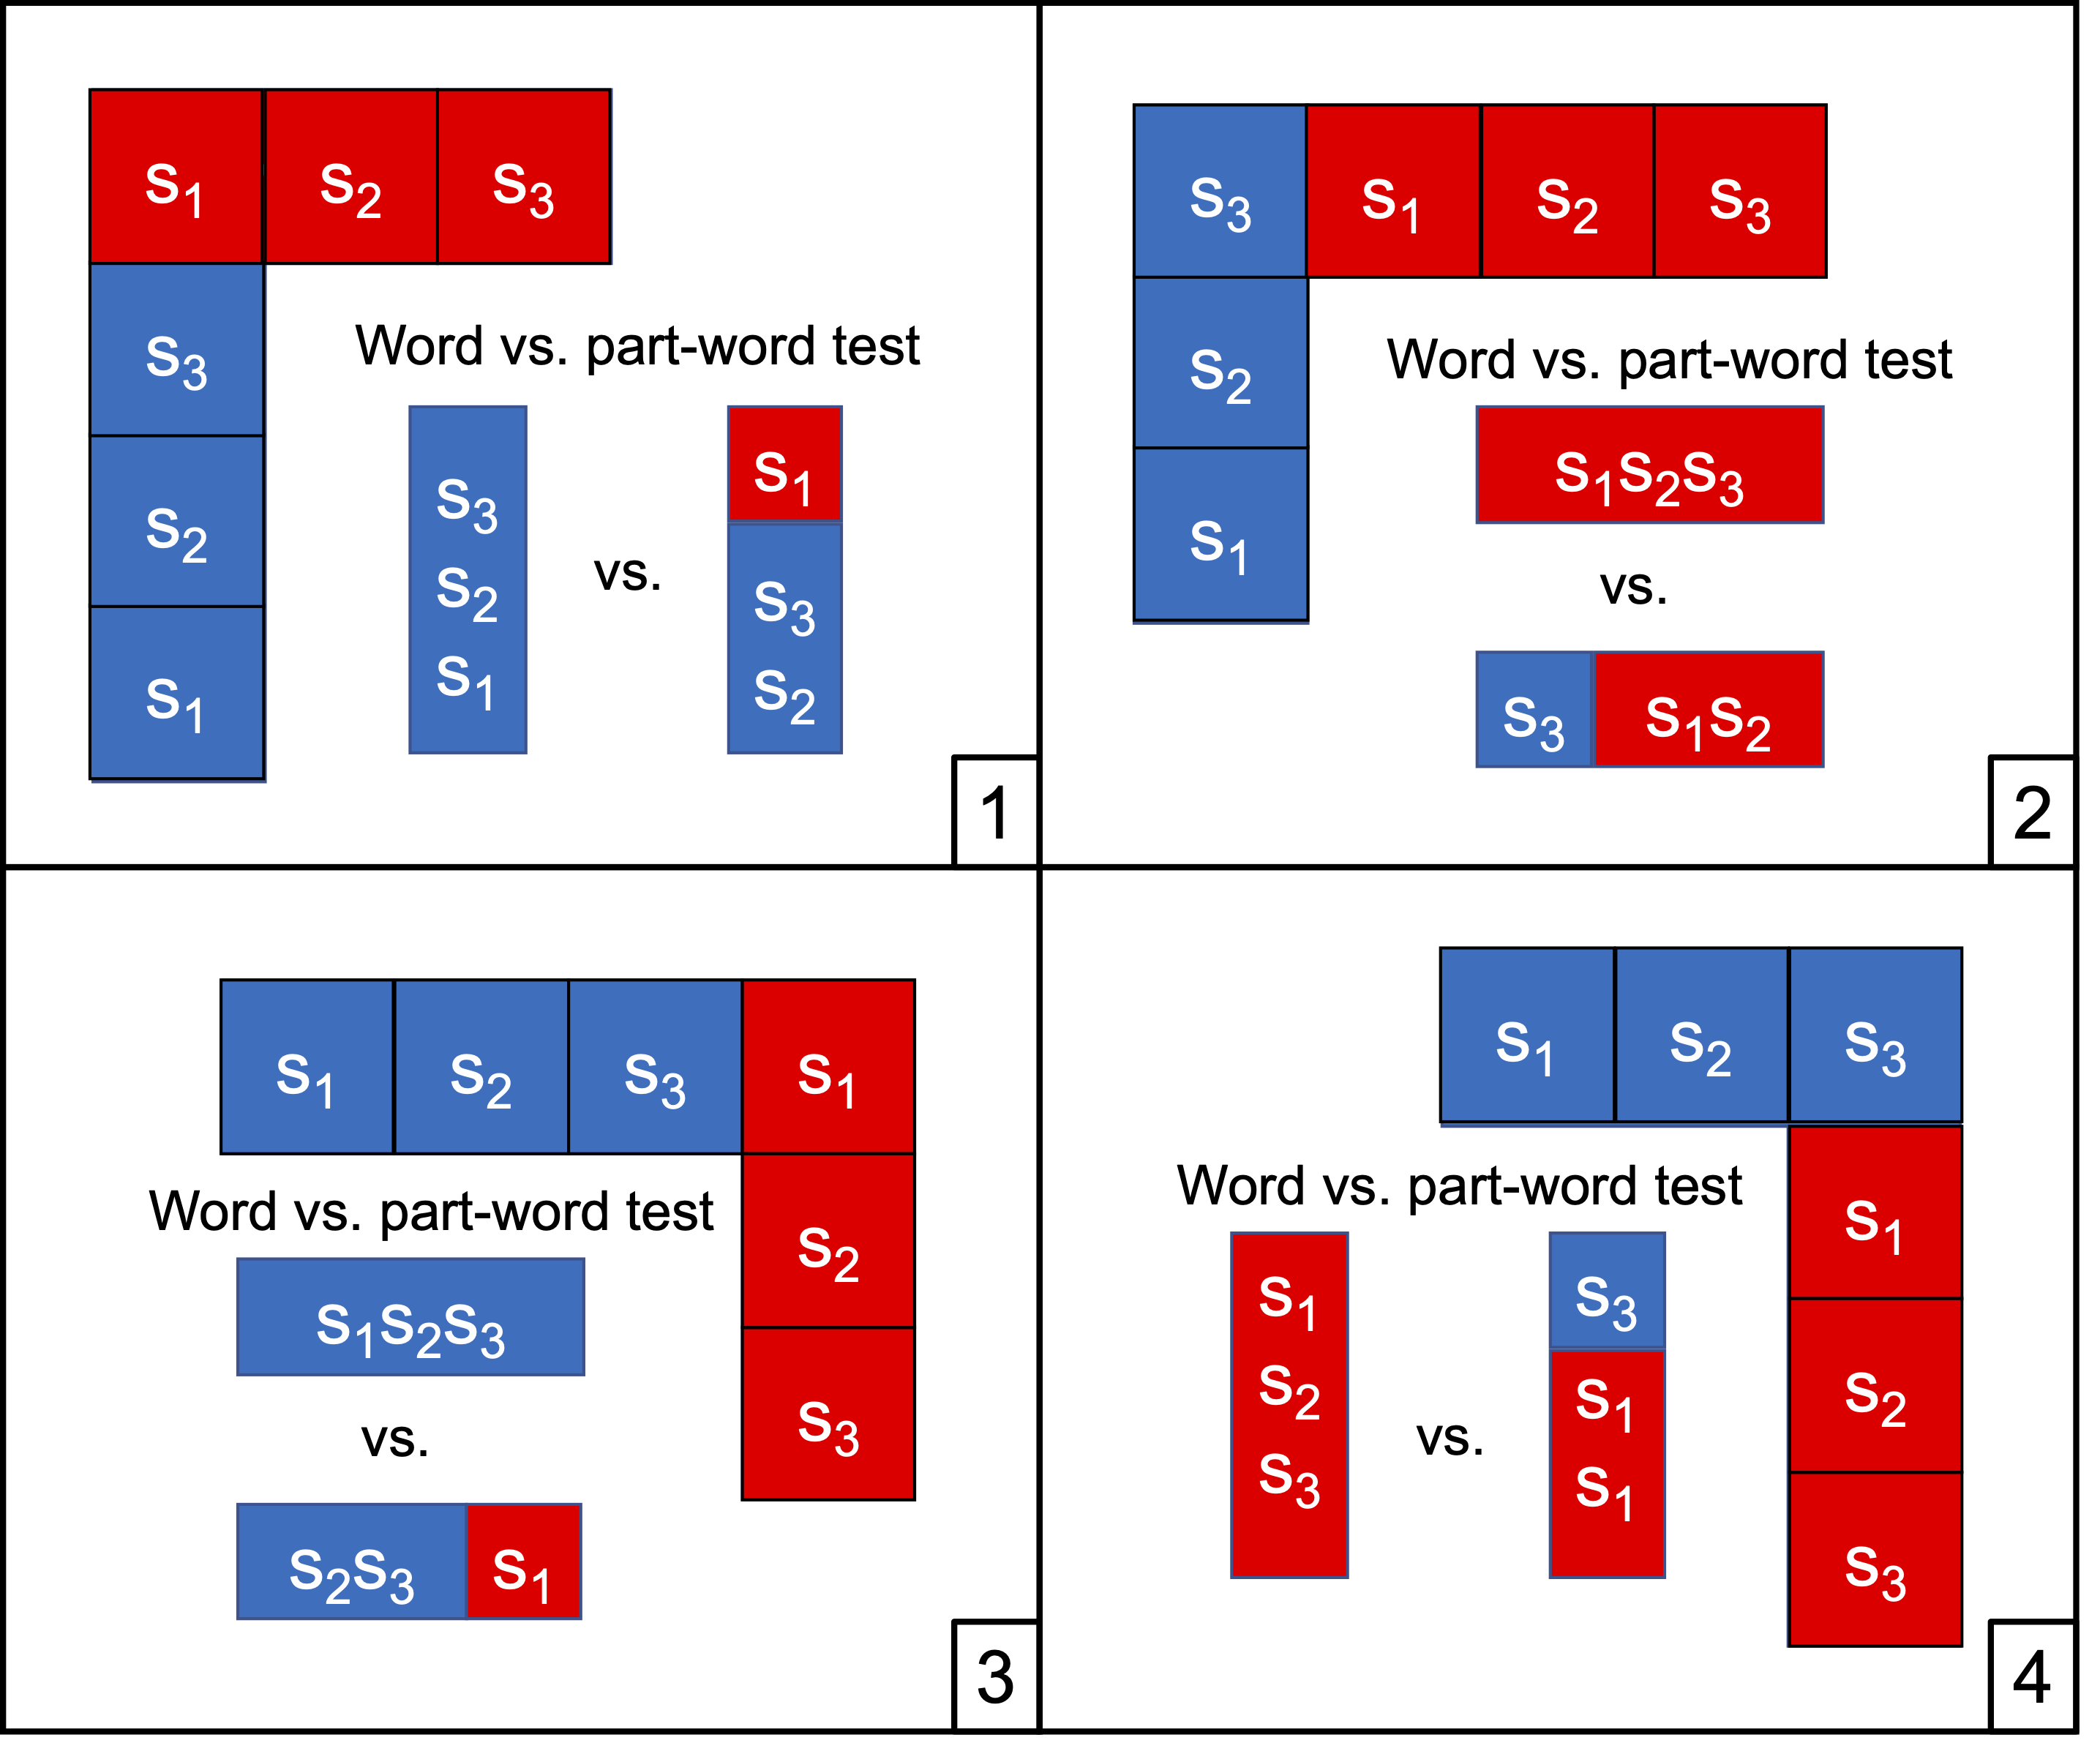
\includegraphics{../figs/configurations.png}
\caption{The basic configurations}
\end{figure}

Compared to the horizontal orientation, vertical shape combinations were
rotated by 90 degrees to the left when the vertical shape combinations
appeared on the left (i.e., in Configurations 1 and 2), and by 90
degrees to the right when the vertical shape combinations appeared on
the right (i.e., in Configurations 3 and 4). The shapes were not
rotated.

\hypertarget{test}{%
\subsection{Test}\label{test}}

\hypertarget{word-vs.-part-word-test}{%
\subsubsection{Word vs.~Part-Word test}\label{word-vs.-part-word-test}}

As shown in the Figure above, each configuration admits exactly one
part-word. For example, in Configuration 1, the only part-word without a
bend uses the two top-most symbols from the vertical word and the
left-most symbol from the horizontal word.

We randomly selected 12 combinations of words of the two sets, which
each word appearing equally often as the first or second word. We
randomly paired these combinations with a configuration and generated
the corresponding words and part-words. Each configuration was used
equally often. As a result, each word occurred twice, and each part-word
once.

Words and part-words were presented centered on the screen rather than
in their original positions. The test items were presented one after the
other. The order was randomly chosen; an equal number of trials started
with words and part-words, respectively.

\hypertarget{word-vs.-phantom-word-test}{%
\subsection{Word vs.~Phantom-word
test}\label{word-vs.-phantom-word-test}}

In the Word vs Phantom-word test, we presented all words and their
corresponding phantom-words. As a result, each word occurred once, and
each phantom-word three times. Orientations are chosen randomly. Items
occur one after another, with the order of items chosen randomly.

\hypertarget{part-word-vs.-phantom-word-test}{%
\subsection{Part-word vs.~phantom-word
test}\label{part-word-vs.-phantom-word-test}}

In the Phantom-Word vs.~part-word test, we reuse the same trials as in
the Word vs.~Part-Word test, except that words are replaced by the
corresponding phantom-words. As a result, each phantom-word occurs 3
times, while each part-word occurs once. In line with Endress \&
Mehler's results, phantom-words are treated as legal items

\hypertarget{print-testable-files}{%
\subsection{Print testable files}\label{print-testable-files}}

  \bibliography{/Users/endress/ansgar.bib}

\end{document}
